% Tipo di documento. L'uso di twoside implica che i capitoli inizino sempre con la prima pagina a sinistra, eventualmente lasciando una pagina vuota nel capitolo precedente. Se questa cosa è fastidiosa, è possibile rimuoverlo. 
% \documentclass[a4paper, twoside,openright]{report}
\documentclass[a4paper,openright]{report}

\usepackage{graphicx} % Required for inserting images
\setkeys{Gin}{width=0.6\textwidth}

\usepackage[utf8]{inputenc}

\usepackage{hyperref}

\usepackage{wrapfig}

\usepackage{enumitem}
\renewcommand{\labelitemi}{$\diamond$}
\renewcommand{\labelitemiii}{$\circ$}
\setlist[enumerate,2]{label=\roman*.}
\setlist[enumerate,3]{label=(\alph*)}

\setitemize{noitemsep}
\setenumerate{noitemsep}
\setlist{noitemsep}

\usepackage{paracol}
\usepackage{multicol}
\usepackage{booktabs}


\usepackage{geometry}

\usepackage{color}

\usepackage{listings}
% \usepackage{minted}

\usepackage{amsmath}
\usepackage{amssymb}
\usepackage{amsfonts}
\usepackage{bm}

\usepackage{wasysym}

% Uso dei colori
\usepackage[dvipsnames,table,xcdraw]{xcolor}
\usepackage{colortbl}
\usepackage{rotating}
\usepackage{adjustbox}

\usepackage{multirow}
\usepackage{soul}
\usepackage{booktabs}
\usepackage{makecell}


\usepackage{tikz}
\usetikzlibrary{automata, arrows,bending}
\usetikzlibrary{positioning}
\usetikzlibrary{shapes.geometric}
\usepackage{parskip}

\usepackage{soul}

% This are needed because the correct double quotes would be ``'' or ``",
% but i've always written "text"
% TODO - check whether this affects listing environment
% \usepackage [english]{babel}
% \usepackage [autostyle, english = american]{csquotes}
% \MakeOuterQuote{"}

\geometry{margin=0.6in}

\setlist[description]{itemsep=0em,topsep=0.5em,parsep=0em}
\setlist[itemize]{itemsep=0em,topsep=0pt}

\hypersetup{
    colorlinks=true,
    linkcolor=black,
    filecolor=mauve,
    urlcolor=blue,
}

\definecolor{gray}{gray}{0.3}
\definecolor{verylightgray}{gray}{0.95}
\definecolor{blue}{rgb}{0,0,1}
\definecolor{mauve}{rgb}{0.58,0,0.82}
\definecolor{darkred}{rgb}{0.3,0,0}
\definecolor{darkgreen}{rgb}{0,0.3,0}
\definecolor{darkgray}{gray}{0.15}



\newenvironment{notes}{
\par
\color{gray}
\small}

\newcommand{\note}[1]{\begin{notes}{#1}\end{notes}}
\newcommand{\nl}[0]{\parskip = \baselineskip}
\newcommand{\lst}[1]{\lstinline{#1}}


\newlength{\currentparindent}
\newcommand{\labelitemize}[2]{
\setlength{\currentparindent}{\parindent}
\setlength{\parindent}{0pt}

\begin{minipage}{0em} % Adjust the width as needed
    \makebox[0em][c]{\rotatebox{90}{\small #1}}
\end{minipage}
\begin{minipage}{\dimexpr\columnwidth-1cm\relax}
    #2
\end{minipage}
\setlength{\parindent}{\currentparindent}
}
\newcommand{\colfill}{\vspace{\fill}}


\lstset{frame=false,
 showstringspaces=false,
 breaklines=true;
 columns=flexible,
 basicstyle={\small\ttfamily},
 keywordstyle=\color{blue},
 commentstyle=\color{dkgreen},
 stringstyle=\color{mauve}
 tabsize=3
}

\title{Mobile and Cyber Physical Systems - Appunti}
\author{Francesco Lorenzoni}
\date{February 2024}

\begin{document}

\maketitle
\tableofcontents

\chapter{Introduction}
\section*{27 - Settembre}
\section{Product based}
In \textit{Project-based SE} there is loop which nowdays cripples software since its early stages of development.
This is due to mutable nature of requirements, which often change throughout time along the features implemented by the software.
\begin{center}
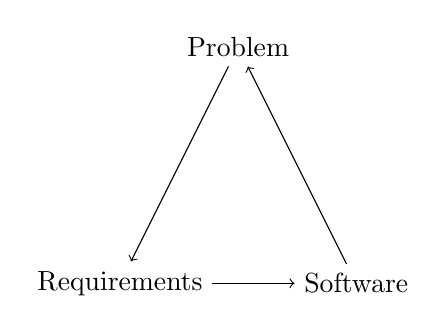
\begin{tikzpicture}
    \node[draw=white,align=left] (A) at (1.5,3) {Problem};
    \node[draw=white,align=left] (B) at (0,0) {Requirements};
    \node[draw=white,align=left] (C) at (3,0) {Software};

    \path [->] (A) edge node[left] {} (B);
    \path [->] (B) edge node[left] {} (C);    
    \path [->] (C) edge node[left] {} (A);    
\end{tikzpicture}
\end{center}

\textit{Product-based SE} is opposed to \textit{Project-based SE} and the above pictures changes as follows.

\begin{center}
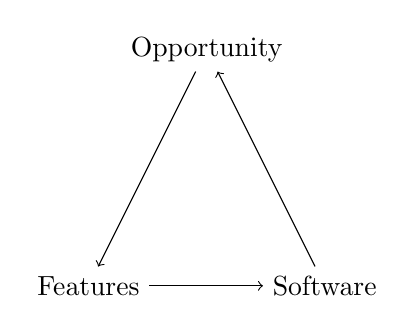
\begin{tikzpicture}
    \node[draw=white,align=left] (A) at (1.5,3) {Opportunity};
    \node[draw=white,align=left] (B) at (0,0) {Features};
    \node[draw=white,align=left] (C) at (3,0) {Software};

    \path [->] (A) edge node[left] {} (B);
    \path [->] (B) edge node[left] {} (C);    
    \path [->] (C) edge node[left] {} (A);    
\end{tikzpicture}
\end{center}

\section{Agile}
Agile is a collection of principles and methods applied in the software development field.
\nl

Opposed to project-based SE, in Agile the client is requested to express the requirements not in technical terms but in features.

Agile suggests an incremental development model

\subsection*{Principles}
\begin{enumerate}
    \label{subsec:agile_principles}
    \item Satisfy customer through early and continuous delivery of valuable software
    \item Welcome changing requirement, even late in development.
    Agile processes harness change for the customer's comptetitive advantage
    \item Deliver working software frequently, from a couple of weeks to a couple of months, with a preference to the shorter timescale
    \item Business people and devs must work together daily throughout the prokect
    \item Build porjects around motivated individuals and give them the environment and support they need
    \item The most efficient and effective method of conveying information to and within a dev team is face-to-face conversation
    \item Working software is the primary measure of progress
    \item Agile processes promote sustainable dev 
    \item Continuous attention to technical excellence and good design enhances agility
    \item Simplicity i.e. art of maximizing the amount of work not done is essential
    \item The best architectures, requirements, and designs emerge from self-organizing teams.
\end{enumerate}

Extreme Programming was proposed as part of the agile methodology

\section{Scrum}
Since requirements changes are rather frequent, long-term plans are unreliable,
hence SE aims to formulate short-term plans.

Scrum is found on \textbf{empiricism} and \textbf{lean thinking}; it asserts that knowledge comes from experience, and that decisions should be made on observations.

Other key terms are code \textbf{Transparency} among the team and with the customer, \textbf{Inspection} of produced code and software (artifacts), \textbf{Adaptation} to changes in features and requirements.

The \textbf{Scrum Team} is composed by:
\begin{enumerate}
    \item \textbf{Product Owner}: must ensure that the dev team is always focused on the goal
    \item \textbf{Scrum Master}: Scrum expert which drives the team to apply properly the Scrum framework.
    \item \textbf{Developers}: actual monkeys people which write code
\end{enumerate}

In scrum SW is developed in \textbf{sprints}, i.e. fixed-length periods with a specific goal to be achieved.

\begin{itemize}
    \item Product backlog: to-do list of items to be implemented
    \item Timeboxed sprints
    \item Self-organizing teams
\end{itemize}

...
\textbf{Prod Backlog Revised}\\
\textbf{PBI Estimation Metrics}

\subsection{Timeboxed Sprints}
Even if at the end of a srpint the goal hasn't been reached, "no worries", the work stops anyway;
there will be a new sprint which will include the work which has not been implemented in the previous one.

\subsection{Scrum Meetings}

\subsection{Agile activities}
Test automation
Continuous integration

\subsection{Sprint reviews}
At the end of each sprint there is a review meeting which involves the \textit{whole} team.
The \textit{product owner} has the ultimate authority to decide wether the sprint goal has been reached or not.
The sprint review should include a process review, in which the whole team shares ideas on how to improve their way of working.

\textbf{Team size}\nl

\section{5 - Ottobre}





\end{document}
